\newpage
\section{Full-Text Search}
Commercial database management has long focused on structured data and the industry requirements have matched those of structured storage applications quite well.
The problem is that only a small part of the data stored is completely structured, while most of it is completely unstructured or only semi-structured, in the form of documents, emails, web pages, etc. \parencite[p. 7]{hamilton_microsoft_2001}\\
\subsection{Microsoft SQL Server Search Architecture}
Text
\begin{figure}[H]
    \caption{Architecture of Microsoft SQL Server Full-Text Search}
    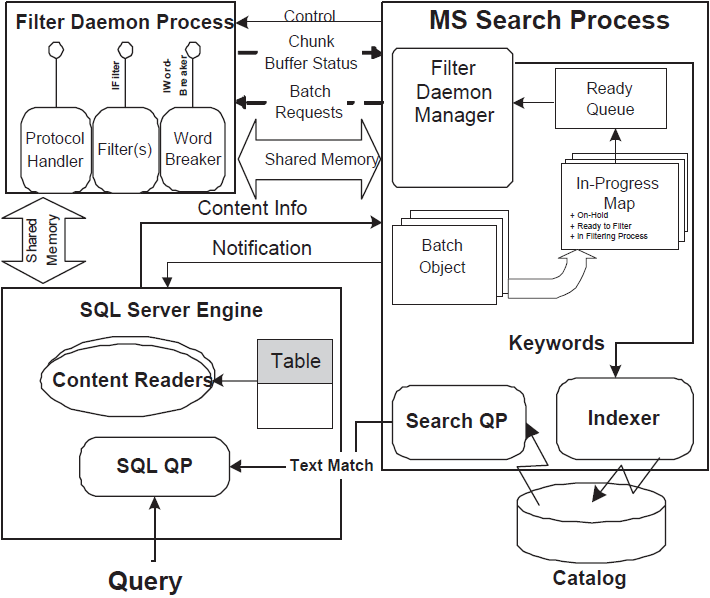
\includegraphics[width=0.9\textwidth]{sql_search_architecture.png}
    \\
    \cite[Source:][p. 8]{hamilton_microsoft_2001}
\end{figure}
More Text